% Auto-generated figure snippets. Embed inline from main.tex.
\begin{figure}[t]
\centering
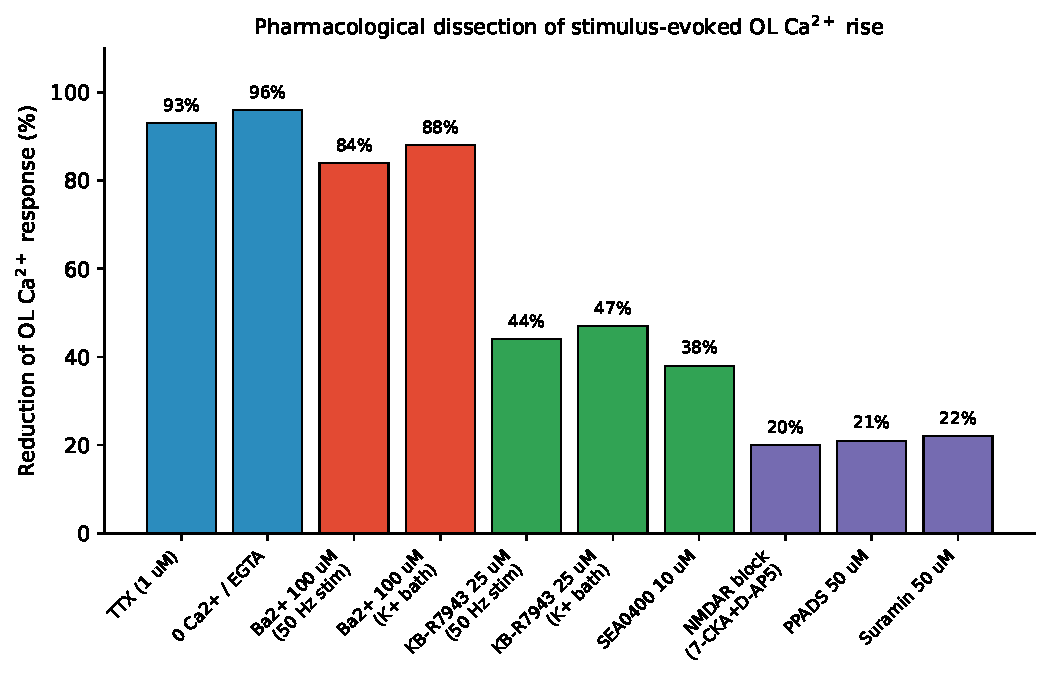
\includegraphics[width=\linewidth]{figures/fig1_drug_effects.pdf}
\caption{Pharmacological dissection of the 50~Hz stimulation-evoked oligodendrocyte (OL) Ca$^{2+}$ response in acute optic nerves. Bars show the percentage reduction of the stimulus-evoked Ca$^{2+}$ area under the curve (AUC) in OL somata upon application of each drug (or high-[K$^+$] bath challenge where indicated). Values are taken from paired recordings across 3--6 nerves per condition; all reductions reach $p<0.005$ in paired $t$-tests unless marked otherwise.}
\label{fig:drug_effects}
\end{figure}

\begin{figure}[t]
\centering
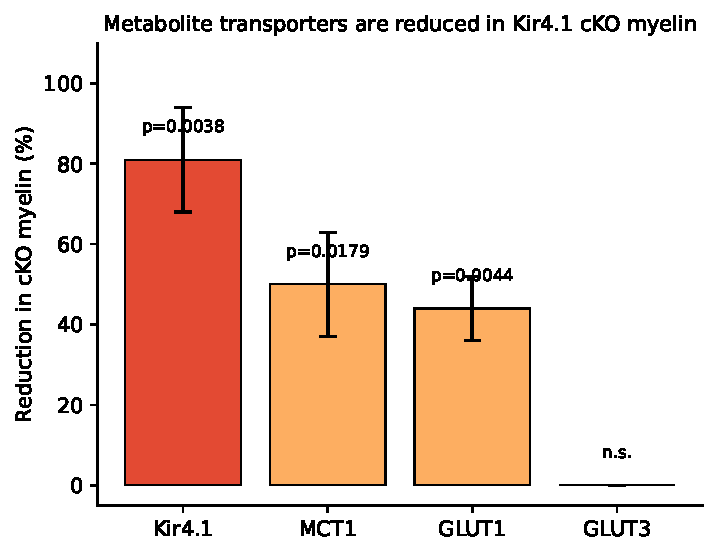
\includegraphics[width=0.7\linewidth]{figures/fig2_myelin_transporters.pdf}
\caption{Immunoblot quantification in biochemically purified central myelin from 2.5-month-old Kir4.1 cKO ($n=3$) versus littermate controls ($n=3$). Kir4.1, MCT1 and GLUT1 are reduced in cKO myelin, while GLUT3 is unchanged (Extended Data Fig.~7).}
\label{fig:myelin_transporters}
\end{figure}

\begin{figure}[t]
\centering
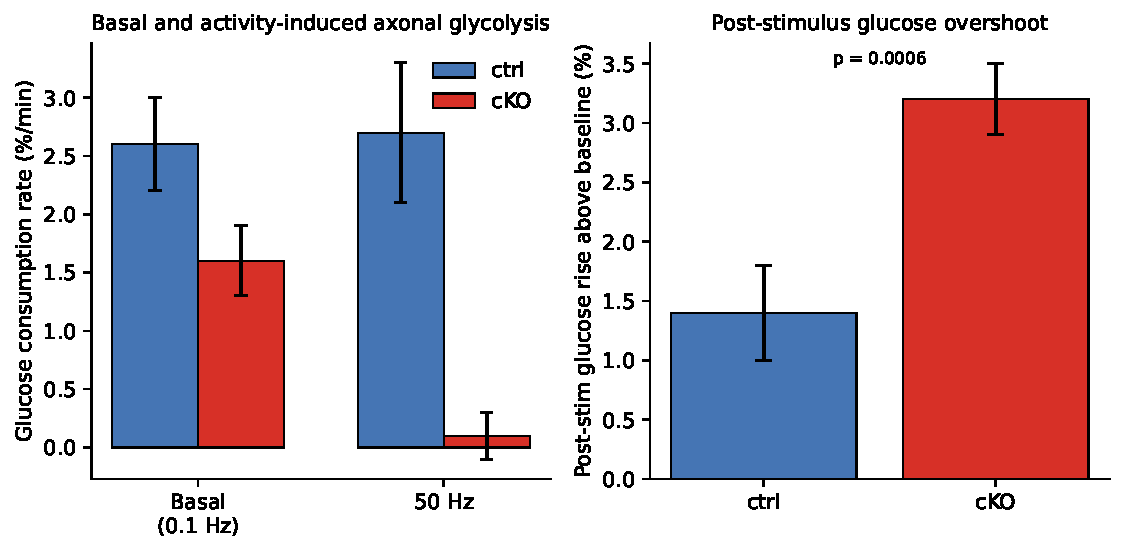
\includegraphics[width=\linewidth]{figures/fig3_axonal_glucose.pdf}
\caption{Axonal glucose dynamics in ctrl and Kir4.1 cKO optic nerves. \textbf{Left}, glucose consumption rate measured with cytochalasin~B at basal 0.1~Hz stimulation and during 50~Hz stimulation. \textbf{Right}, post-stimulation overshoot of axonal glucose, consistently elevated in cKO.}
\label{fig:axonal_glucose}
\end{figure}

\begin{figure}[t]
\centering
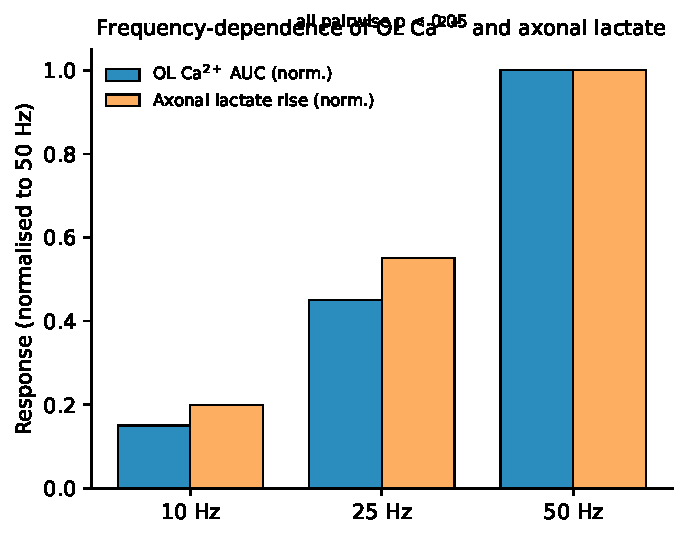
\includegraphics[width=0.65\linewidth]{figures/fig4_frequency_dependence.pdf}
\caption{Frequency dependence of the OL Ca$^{2+}$ surge and the axonal lactate rise evoked by 30~s trains at 10, 25 and 50~Hz. Values are normalised to the 50~Hz condition; all pairwise comparisons reached $p<0.05$ (one-way ANOVA with Tukey's or Holm-\v{S}{\'i}d{\'a}k's post-hoc).}
\label{fig:freq_dependence}
\end{figure}

\begin{figure}[t]
\centering
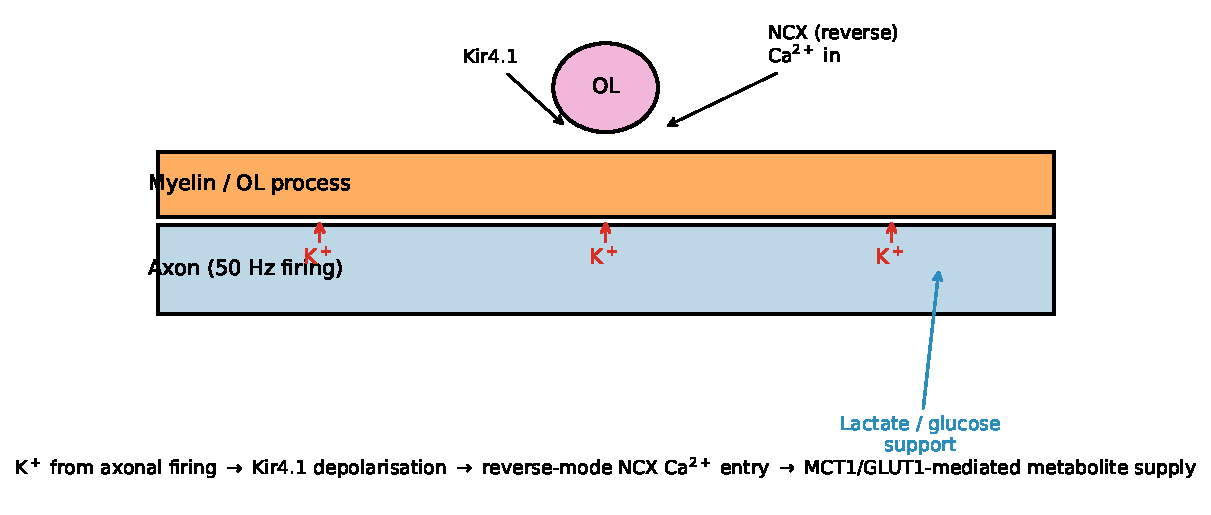
\includegraphics[width=\linewidth]{figures/fig5_working_model.pdf}
\caption{Working model: high-frequency axonal firing elevates periaxonal [K$^+$], depolarising oligodendrocytes through Kir4.1. Depolarisation activates reverse-mode Na$^+$/Ca$^{2+}$ exchanger, raising somatic Ca$^{2+}$. Kir4.1-dependent signalling supports the abundance of MCT1 and GLUT1 in myelin, coupling axonal firing to activity-induced lactate and glucose supply.}
\label{fig:working_model}
\end{figure}
